\part{Construction du modèle}
    \chapter{Les principes généraux}
        \section{Contenu du texte d'une liste d'ingrédients}

        En général, chaque ingrédient sera présent une seule fois dans la liste (cf. section \mref{listes_ingredients})

        Le calcul d'embeddings via des modèles tels que SVD ou Word2Vec fait peu de sens.
        \newline
        \newline
        \emphbox{l'extraction des textes se fait au format \emph{Bag Of Words}, sans utiliser de notion d'IDF. L'utilsation de TF semble églament ne pas amener de valeur à priori.}

        \section{Limitation à l'identification des listes d'ingrédients}

        On est sur une taxonomie d'informations limitée dans les fiches techniques.

        On pourrait envisager de classifier l'ensemble des textes présents dans les fiches techniques.

        Mais l'absence de données étiquetées rend cette tâche impossible. La charge d'étiquetage d'un nombre représentatif de blocs de texte de fiches techniques est trop importante pour être mise en oeuvre dans le cadre de ce projet.

        \section{Conversion de documents en texte}
        
        dire ici qu'on utilise principalement pdfminer vs. d'autres outils d'OCR.

        De plus, on partira dans un premier temps sur une transformation basique d'un document en texte, sans passer par une analyse de la localisation des textes sur le document (cf. les difficultés présentées dans la section \mref{formats_spatialisation}).
            
    \chapter{Construction d'un modèle simple \og ouvert \fg}
        
        \section{Principes généraux}

            \begin{figure}[htbp]
                \begin{center}
                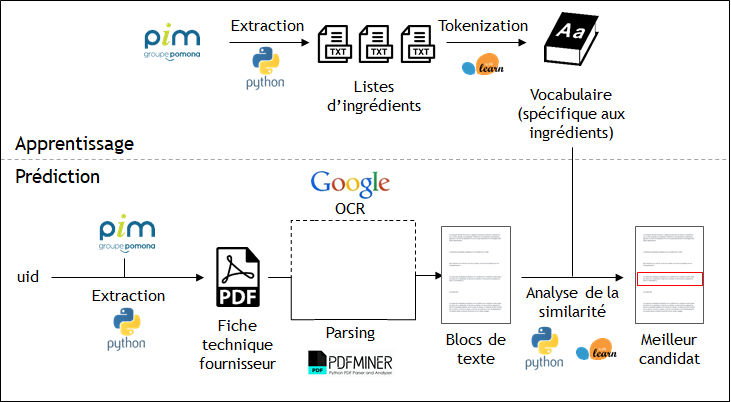
\includegraphics[width=0.9\linewidth]{img/open_model.png}
                \end{center}
                \caption{Schéma de principe du \og modèle ouvert \fg}
                \label{fig:open_model}
            \end{figure}     

            Le fonctionnement global de ce premier modèle (présenté à la \reffig{fig:open_model}) ne respecte pas les principes du machine learning.
            Il permet juste d'éprouver la méthode pressentie, ainsi que de se faire une idée de l'efficacité d'un modèle de ce type.
            En effet, même si on utilise des fonctionnalités d'extraction de features depuis des textes classiques dans des modèles de machine learning, il manque une partie de mesure de la performance, indispensable pour pouvoir évaluer et améliorer la pertinence du modèle.
            Les illustrations de ce chapitre sont issues du notebook présenté en annexe \mref{code:open_model}, et le code des classes utilisées (IngredientExtractor et PIMIngredientExtractor) est inclus dans le module pimest, en annexe \mref{code:pimest}.

            La classe PIMIngredientExtractor est juste un habillage du CountVectorizer de la bibliothèque scikit-learn et du Requester construit dans le module pimapi, permettant d'aller récupérer les données du PIM.
            Ce modèle met en application les principes du \og Bag Of Words \fg \cite{bag_of_words_wiki}, à savoir que :
            \begin{itemize}
                \item un vocabulaire est établi à partir de l'ensemble des différents mots du corpus de listes d'ingrédients
                \item chaque liste d'ingrédients est transformée en un vecteur de nombres entiers qui a la même longueur que le vocabulaire, ou chaque entier est le compte du nombre d'occurence du mot dans le vocabulaire
            \end{itemize}

            Ce modèle n'utilise pas les données étiquetées manuellement (présentées à la section \mref{manually_labelled_data}), mais se base simplement sur les listes d'ingrédients du PIM.
            L'hypothèse qui est faite avec ce modèle est la suivante : bien que non parfaitement en qualité (i.e. exactement identiques au contenu des pièces jointes, cf. la comparaison entre la ground truth et le contenu du PIM en section \mref{ingredient_comparison}), les listes d'ingrédients du PIM sont des textes dont le contenu est très similaire à une liste d'ingrédients.
            Un survol rapide de quelques exemples montre que cette hypothèse semble vérifiée (cf. \reftable{tbl:exemple_ingred}).

        \section{Entraînement}

            \subsection{Périmètre du set d'entraînement}
            
            Pour l'entraînement de ce modèle, on va uniquement se limiter aux produits d'épicerie ou de boissons non-alcoolisées.
            En effet, ce sont pour ces produits que la réglementation impose d'afficher en clair la composition aux consommateurs.
            On se limitera aussi aux produits qui portent une liste d'ingrédients, et qui sont \og En qualité \fg (cf. les définitions données à la section \mref{statuts} sur les statuts des produits).
            Sur les 13 000+ produits présents dans le PIM, environ 3 400 font partie du périmère et 9 800 en sont exclus.

            \subsection{Constitution du vocabulaire}

            La constitution du vocabulaire se fait de manière très basique : 
            \begin{itemize}
                \item les listes d'ingrédients sont mises en minuscules
                \item les mots sont ensuite séparés aux whitespaces (espaces, retours à la ligne, tabulations, \dots) et marques de ponctuation
            \end{itemize}
            Pour parvenir à ce résultat, on applique simplement la méthode fit de la classe CountVectorizer de la bibliothèque scikit-learn.
            Aucunes des autres fonctionnalités standard (retrait des accents, gestion des stopwords) n'a été activée.
            Lors de cet apprentissage, le vocabulaire obtenu a une longueur de 2 500 mots environ, et les mots les plus fréquents sont :
            \begin{itemize}
                \item de     : 11419 occurences
                \item sucre  :  2057 occurences 
                \item sel    :  1669 occurences
                \item eau    :  1288 occurences
                \item acide  :  1241 occurences
                \item lait   :  1215 occurences
                \item huile  :  1214 occurences
                \item poudre :  1100 occurences
                \item en     :   962 occurences
                \item arôme  :   938 occurences
            \end{itemize}
            (ces valeurs sont susceptibles de changer à la marge par rapport au notebook en annexe, avec les changements potentiels sur les données au sein du PIM)
            Les stopwords 'de' et 'en' apparaissent dans les mots les plus fréquents.        
        
        \section{Prédiction}
            
            \subsection{Parsing des fiches techniques}

                Les fiches techniques sont extraites sous formes de binaires depuis de le PIM via des appels API.
                On utilise ensuite la bibliothèque PDFMiner.six pour récupérer le texte de la fiche technique sous forme d'un long string.
                Cette étape fait appel à la méthode statique PDFDecoder.content du module pimpdf, présenté en annexe \mref{code:pimpdf}.
                On découpe ensuite ce long string en une liste de string plus court, en considérant comme séparateur la présence de deux retours à la ligne consécutifs.
                Ce choix de séparateur a été fait car les textes produits par PDFMiner.six portent des retours à la ligne à la fin de chaque ligne typographiée, même si la phrase continue sur la ligne suivante.
                Cette étape fournit pour chaque fiche technique le texte contenu sous forme d'une liste de strings (les blocs de texte de la \reffig{fig:open_model}).

            \subsection{Sélection du meilleur candidat}

                \subsubsection{Principe}
                L'identification du meilleur candidat parmi les blocs de texte se fait de la manière suivante :
                \begin{itemize}
                    \item on calcule une similarité avec le vocabulaire des ingrédients pour chacun des blocs de texte
                    \item on retourne le bloc de texte avec la similarité la plus élevée
                \end{itemize}
                La formule de calcul de la similarité utilisée dans ce modèle a été trouvée par chance (ou plutôt par erreur, pour être honnête).
                Néanmoins, elle donne des résultats plutôt encourageants.
                D'autres modes de calcul de la similarité seront présentés dans la suite de ce rapport.

                La formule de calcul de la similarité est :
                \[\frac{\text{Nombre de mots du candidat qui sont des ingrédients}}{\text{Norme euclidienne du vecteur du candidat}}\]
                
                Attention, la norme du vecteur du candidat s'entend \emph{indépendamment du vocabulaire des ingrédients}, c'est à dire que tous les mots comptent, y compris ceux n'appartenant pas au vocabulaire.

                \subsubsection{Exemple}
                Si on illustre par un exemple fictif : imaginons que le vocabulaire des ingrédients soit composé des mots \emph{\og eau \fg, \og sucre \fg et \og farine \fg}.
                Le bloc de texte candidat est \emph{\og Sucre et farine sont biologiques. La farine est équitable.\fg}
                Si on vectorise ce bloc de texte \emph{sur son propre vocabulaire}, on obtient le vecteur suivant : 

                \bigskip
                \begin{minipage}{\textwidth}
                \captionsetup{type=table}
                \centering
                \begin{tabular}{cccccccc}
                    \toprule
                    sucre & et & farine & sont & biologiques & la & est & équitable \\
                    \midrule
                    1 & 1 & 2 & 1 & 1 & 1 & 1 & 1 \\
                    \bottomrule
                \end{tabular}
                \caption{Exemple de vectorisation d'un texte}
                \bigskip
                \end{minipage}                

                Sa norme euclidienne~\cite{norm_wiki} se calcule de la manière suivante (en notant $x_{i}$ le compte des mots) : 
                \[\sqrt{\sum_{i}^{} x_{i}^{2}} = \sqrt{1 + 1 + 4 + 1 + 1 + 1 + 1 + 1} \approx 3.317\]

                Le bloc contient 9 mots, dont 3 sont des ingrédients (\og farine \fg est mentionné deux fois). La similarité pour cet exemple vaut donc :
                \[\frac{3}{3.317} \approx 0.905\]
                \'{E}tant donné son mode de calcul, cette similarité peut tout à fait être supérieure à 1.

        \section{Illustration des résultats obtenus}
    
            \subsection{Périmètre du test}
            
            Pour éviter de surestimer la performance du modèle, on le fait tourner sur des produits n'ont pas fait partie du set d'entraînement.            
            Comme ce modèle ne permet de toute façon pas de fournir de résultats qui permettent de mesurer la performance, on ne le fera tourner que sur un échantillon réduit de produits, soit 5 d'entre eux.

            \subsection{Résultats}

            Les résultats obtenus sont les suivants :

                \begin{spacing}{1.0}
                \label{blocks_examples}
                {\scriptsize
                {\ttfamily 
                \begin{spverbatim}
Fetching data from PIM for uid d9b233a6-b455-4af6-afb4-623f1f7f62a6...
Done
----------------------------------------------------------
Ingredient list from PIM is :

Ingrédients: Huile de tournesol, oignon, curry (11,2%) (ail, coriandre, curcuma, gingembre, paprika, poivre, cumin, poivre de Cayenne, fenouil, cardamome, noix de muscade, canelle, clous de girofle, safran), pomme, sel, exhausteur de goût (glutamate de sodium), sucre, huile de colza totalement hydrogénée, extrait de levure, ail.
----------------------------------------------------------
Downloading content of technical datasheet file...
Done!
----------------------------------------------------------
Parsing content of technical datasheet file...
Done!
----------------------------------------------------------
Ingredient list extracted from technical datasheet:

Liste d’ingrédients : Huile de tournesol, oignon, curry (11,2%) (ail, coriandre, curcuma, gingembre, paprika, poivre, cumin,
poivre de Cayenne, fenouil, cardamome, noix de muscade, canelle, clous de girofle, safran), pomme, sel, exhausteur de goût
(glutamate de sodium), sucre, huile de colza totalement hydrogénée, extrait de levure, ail
----------------------------------------------------------

=======================================================================
=======================================================================
Fetching data from PIM for uid 5666235b-9e78-44f2-8e0e-1de53f88fe04...
Done
----------------------------------------------------------
Ingredient list from PIM is :

Ingrédients : Sucre, Gomme base, Sirop de glucose, Arômes, Humectant (E422), Antioxydant (E321), Colorant (E141).
----------------------------------------------------------
Downloading content of technical datasheet file...
Done!
----------------------------------------------------------
Parsing content of technical datasheet file...
Done!
----------------------------------------------------------
Ingredient list extracted from technical datasheet:

INGRÉDIENTS : Sucre, Gomme base, Sirop de glucose, Arômes, Humectant (E422), 
Antioxydant (E321), Colorant (E141).
----------------------------------------------------------

=======================================================================
=======================================================================

Fetching data from PIM for uid 6e976147-adeb-4d2d-925a-cb7c58c111a2...
Done
----------------------------------------------------------
Ingredient list from PIM is :

Maltodextrine, amidon de maïs, sel, farine de BLE, colorant : caramel ordinaire ; arômes (BLE,CELERI), huile de palme, épaississant : gomme guar ; oignon, fécule de pomme de terre, extrait de levure, jus de cuisson de viande de boeuf (0,9%), acidifiant : acide citrique ; extrait de vin blanc, extraits d'ail, de thym et de poivre. Peut contenir : LAIT, OEUF.
----------------------------------------------------------
Downloading content of technical datasheet file...
Done!
----------------------------------------------------------
Parsing content of technical datasheet file...
Done!
----------------------------------------------------------
Ingredient list extracted from technical datasheet:

Maltodextrine, amidon de maïs, sel, farine de blé, colorant : caramel ordinaire ; arômes (blé,céleri), huile de palme, épaississant : gomme guar ; oignon, fécule 
de pomme de terre, extrait de levure, jus de cuisson de viande de bœuf (0,9%), acidifiant : acide citrique ; extrait de vin blanc, extraits d'ail, de thym et de poivre. 
Peut contenir : lait, œuf.

----------------------------------------------------------

=======================================================================
=======================================================================

Fetching data from PIM for uid db449562-d16d-4f72-b7a5-c0d487bc8206...
Done
----------------------------------------------------------
Ingredient list from PIM is :

Huile d'ARACHIDE

----------------------------------------------------------
Downloading content of technical datasheet file...
Done!
----------------------------------------------------------
Parsing content of technical datasheet file...
Done!
----------------------------------------------------------
Ingredient list extracted from technical datasheet:

*Selon le règlement UE n°1259-2011 / In accordance with regulation UE n°1259-2011  
    
    
CARACTERISTIQUES MICROBIOLOGIQUES 
    
L’huile étant un milieu anhydre, tout développement bactérien est impossible (cf. ouvrage de 
référence  dans  ce  domaine  "La  qualité  microbiologique  des  aliments"  CNERMA-CNRS 
coordonné par Jean-louis Jouve). 
    
ORIGINES/ ORIGIN 
    
- Amérique du Sud majoritairement 
- Afrique de l’Ouest 
    
AUTRES INFORMATIONS 
    

----------------------------------------------------------

=======================================================================
=======================================================================

Fetching data from PIM for uid f2af54a2-6820-4f1b-99e7-d6e64642bdf3...
Done
----------------------------------------------------------
Ingredient list from PIM is :

None

----------------------------------------------------------
Downloading content of technical datasheet file...
Done!
----------------------------------------------------------
Parsing content of technical datasheet file...
Done!
----------------------------------------------------------
Ingredient list extracted from technical datasheet:

mini 16,56 ( - 10 % )

----------------------------------------------------------

=======================================================================
=======================================================================  
                \end{spverbatim}
                }
                }
                \end{spacing}

            \subsection{Pistes d'améliorations identifiées}

            En plus de la mesure de la performance, qui est indispensable avant de pouvoir procéder à des ajustements, les pistes identifiées à sont les suivantes :
            \begin{itemize}
                \item Faire un découpage plus élaboré du texte des pièces jointes en blocs, potentiellement avec des expressions régulières
                \item Faire des \og ngrams de blocs \og, ce qui permettrait de parfois fusionner des blocs qui ont été séparés (car contenaient des retours à la ligne successifs)
                \item Essayer une autre manière de calculer la similarité
                \item \dots
            \end{itemize}

    \chapter{Utilisation des données manuellement étiquetées}

    Comme présenté à la section\mref{ingredient_comparison} relative à la comparaison entre les données du PIM et celles récupérées lors de l'étiquetage, il y a un grand nombre d'écarts.
    Or, si on entraîne le modèle et qu'on mesure sa performance sur des données de mauvaise qualité, on aura de mauvais résultats.
    On va donc construire un modèle se basant sur les données manuellement étiquetées.
    Le fonctionnement de ce modèle est présentés à la \reffig{fig:ground_truth_model}.
    La méthodologie utilisée à cette partie est présentée dans le notebook \og Modèle basé sur les données manuellement étiquetées \fg en annexe \mref{code:gt_based_model}.
    Les différents transformateurs et estimateurs spécifiques sont définis dans le module pimest, inclu en annexe \mref{code:pimest}.
    
    \begin{figure}[htbp]
        \begin{center}
        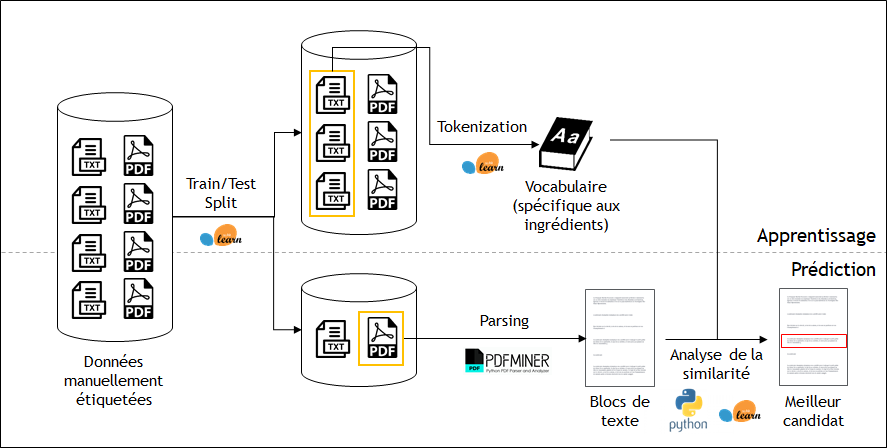
\includegraphics[width=0.9\linewidth]{img/ground_truth_model.png}
        \end{center}
        \caption{Schéma de principe du modèle basé sur les données étiquetées}
        \label{fig:ground_truth_model}
    \end{figure}     

        \section{Chargement des données manuellement étiquetées}

        La toute première étape est la constution d'un dataframe contenant : 
        \begin{itemize}
            \item les uid pour indexer les produits
            \item les listes d'ingrédients manuellement étiquetées depuis les fiches techniques
            \item le contenu de chacune des fiches techniques au format texte
        \end{itemize}
        On commence par charger les données du fichier csv contenant les uid et les listes d'ingrédients.
        Ensuite, un pipeline scikit learn d'acquisition des données est lancé.
        Il s'agit de 3 transformateurs en série, qui effectuent les travaux suivants :
        \begin{itemize}
            \item construction du chemin pointant vers les fiches techniques (sur la base des uid)
            \item construction d'une feature contenant les données des fichiers, en binaire
            \item construction du texte complet de la fiche technique (en se basant sur la library pdfminer.six)
        \end{itemize}
        Le résultat du lancement de ce pipeline est présenté à la \reftable{tbl:mod_GT_fulltexts}.

        {\renewcommand{\arraystretch}{1.5}%
        \begin{table}[htbp]
            \begin{center}
            {\scriptsize
            \begin{tabular}{p{\linewidth}}
\toprule
                                                                                                                                                                                                                                                                                                                                                                                                                                                                                                                                                                                                                                                                                                                                                                                                                                                                                                                                                                                                                                    text \\
\midrule
 NESCAFÉ® SPÉCIAL FILTRE\textbackslash n\textbackslash nDose individuelle de 2 g\textbackslash nTechnologie micro-grains\textbackslash n\textbackslash nCODE EAN (UC)\textbackslash n\textbackslash n3033710076017\textbackslash n\textbackslash nDENOMINATION LEGALE DU PRODUIT\textbackslash n\textbackslash nDESCRIPTION DU PRODUIT\textbackslash n\textbackslash nCafé instantané et café torréfié moulu.\textbackslash n\textbackslash nUne dominante Arabica pour l'arôme et une pointe de Robusta pour le \textbackslash ncorsé, associés à une torréfaction légère pour un café équilibré et peu \textbackslash namer.\textbackslash nSachet dose pour une tasse.\textbackslash n\textbackslash nDOSAGE PRECONISÉ\textbackslash n\textbackslash nMODE OPERATOIRE\textbackslash n\textbackslash nPour obtenir\textbackslash n\textbackslash n1 café Court (DA)\textbackslash n\textbackslash n1 café Long (DA)\textbackslash n\textbackslash nEau\textbackslash n\textbackslash n7\textbackslash n\textbackslash n12\textbackslash n\textbackslash ncl\textbackslash n\textbackslash ncl\textbackslash n\textbackslash nNESCAFÉ®\textbackslash n\textbackslash n SPÉCIAL FILTRE\textbackslash n\textbackslash n2\textbackslash n\textbackslash n2\textbackslash n\textbackslash ng\textbackslash n\textbackslash ng\textbackslash n\textbackslash nA reconstituer avec de l'eau. \textbackslash nTempérature de l'eau : 75°C\textbackslash nPour une qualité optimale, utilisez de l'eau filtrée.\textbackslash n\textbackslash nIngrédients : Café instantané, café torrefié moulu (3\%).\textbackslash n\textbackslash nINGRÉDIENTS\textbackslash n\textbackslash nPROFIL GUSTATIF\textbackslash n\textbackslash nIntensité\textbackslash n\textbackslash nConditionné sous atmosphère protectrice.\textbackslash n\textbackslash nENGAGEMENT QUALITÉ\textbackslash n\textbackslash n- NESTLÉ a un système de management de la qualité, le NMS (NESTLÉ \textbackslash nManagement System), en cohérence avec les systèmes ISO 9001 ... \\
 LENTILLES BLONDES 4mm\textbackslash n\textbackslash nRéférence PQG007-3.22.1\textbackslash nVersion\textbackslash nDate d'application :\textbackslash nPage 1/2\textbackslash n\textbackslash nG\textbackslash n\textbackslash n15/10/2019\textbackslash n\textbackslash nPrésentation\textbackslash n\textbackslash nCaractéristi -\textbackslash n\textbackslash nques \textbackslash n\textbackslash nphysico-\textbackslash nchimiques \textbackslash n\textbackslash nDéfinition\textbackslash n\textbackslash nOrigine\textbackslash nDénomination \textbackslash nlégale\textbackslash n\textbackslash nLentilles de couleur brun clair. Elles sont de forme biconvexe et \textbackslash npossèdent une peau assez épaisse. Leur diamètre est compris \textbackslash nentre 4mm et 5mm\textbackslash n\textbackslash nChine, Canada, France, Italie, USA, Turquie\textbackslash n\textbackslash nLentilles blondes\textbackslash n\textbackslash nProcess\textbackslash n\textbackslash nNettoyage, épierrage, triages\textbackslash n\textbackslash nConservation\textbackslash n\textbackslash n36 mois à l'abri de la chaleur et de l'humidité\textbackslash n\textbackslash nCritères d'analyses\textbackslash n\textbackslash nMoyenne/Tolérance\textbackslash n\textbackslash nMéthodes\textbackslash n\textbackslash nHumidité\textbackslash nMatières minérales étrangères\textbackslash nMatières végétales étrangères\textbackslash nGraines\textbackslash n\textbackslash nImpropres\textbackslash nBrisées\textbackslash nGermées\textbackslash n\textbackslash nCalibre 4-5 mm\textbackslash n\textbackslash n11,5\% / 16\%max\textbackslash n0,05\% / 1\%max\textbackslash n0,15\% / 0,5\%max\textbackslash n\textbackslash n0,5\% / 1\%max\textbackslash n0,4\% / 1\%max\textbackslash n0,05\% / 1\%max\textbackslash n95\% / 90\%min\textbackslash n\textbackslash nNF V03707\textbackslash n\textbackslash nMicrobiologie\textbackslash n\textbackslash nIl n'existe pas de réglementation concernant les exigences microbiologiques \textbackslash npour ce produit.\textbackslash n\textbackslash nPesticides\textbackslash nMét... \\
 FICHE TECHNIQUE \textbackslash n\textbackslash nPRODUIT FINI\textbackslash n\textbackslash n000100\textbackslash n\textbackslash nPurée de Poire Sans Sucres Ajoutés\textbackslash n\textbackslash nDate d'application: 05/05/2014\textbackslash n\textbackslash nPage: 1/2\textbackslash n\textbackslash nCoupelles Aluminium 120 x 95 g\textbackslash n\textbackslash nDéfinition\textbackslash n\textbackslash nCe produit est une purée de fruits obtenue à partir des parties comestibles des fruits (après broyage et sans \textbackslash nconcentration notable).\textbackslash nCe produit est sans sucres ajoutés: il contient uniquement les sucres naturellement présents dans les fruits.\textbackslash nLa purée présente une texture homogène et légèrement granuleuse.\textbackslash n\textbackslash nLa stabilité du produit est obtenue par pasteurisation et dosage à chaud.\textbackslash n\textbackslash nAspects nutritionnels\textbackslash n\textbackslash nDésignation et liste des ingrédients\textbackslash n\textbackslash nValeurs nutritionnelles (pour 100 g)\textbackslash n\textbackslash nDésignation légale :\textbackslash n\textbackslash nPurée de Poires sans sucres ajoutés *\textbackslash n* Contient les sucres naturellement présents dans \textbackslash nles fruits\textbackslash n\textbackslash nListe des ingrédients :\textbackslash n\textbackslash nPoire 99,9\%, antioxydant: acide ascorbique.\textbackslash n\textbackslash nMatières grasses\textbackslash n\textbackslash nEnergie\textbackslash n\textbackslash n65 kcal\textbackslash n\textbackslash n273 kJ\textbackslash n\textbackslash ndont acides gras saturés\textbackslash n\textbackslash nGlucides\textbackslash n\textbackslash nFibres alimentaires\textbackslash nPro... \\
\bottomrule
\end{tabular}

            }
            \caption{Exemples du contenu de fiches techniques au format texte (tronqués)}
            \label{tbl:mod_GT_fulltexts}
            \end{center}
        \end{table}
        }        

        \section{Découpage des textes en blocs}

        Le second travail est le découpage des textes en blocs. 
        Dans un premier temps, on va simplement effectuer ce découpage en splittant le texte lorsque deux retours à la ligne successifs sont détectés.
        Un exemple de découpage est présenté ci-dessous.

        \begin{multicols}{3}
        \begin{spacing}{1.0}
        \label{blocks_examples}
        {\tiny
        30/12/19 \newline -------------------------------------------------------------------- \newline Date d'impression :  \newline Remarque :  \newline Les informations contenues dans cette fiche technique sont données de bonne foi, en l’état actuel de nos connaissances, et selon  \newline les indications communiquées par le producteur ou le fournisseur. Il appartient au client de vérifier la conformité de la marchandise  \newline par rapport à l’usage qu’il en fait. \newline -------------------------------------------------------------------- \newline Création :  \newline -------------------------------------------------------------------- \newline 12/06/12 \newline -------------------------------------------------------------------- \newline 12 rue René Cassin \newline 37390 NOTRE DAME \newline -------------------------------------------------------------------- \newline Tél : \newline 02 47 85 55 00 \newline Fax :02 47 41 33 32 \newline -------------------------------------------------------------------- \newline FICHE TECHNIQUE \newline -------------------------------------------------------------------- \newline Mélange du trappeur, 70 g \newline Trapper blend, 70g \newline -------------------------------------------------------------------- \newline Code article KEREX \newline Nom latin (si disponible) \newline / EAN Code \newline Code barre  \newline -------------------------------------------------------------------- \newline / KEREX Code \newline -------------------------------------------------------------------- \newline / (Latin name) \newline -------------------------------------------------------------------- \newline TEEPTRAPPEUR \newline X \newline 3760063322262 \newline -------------------------------------------------------------------- \newline Poids net \newline Poids brut \newline Origine  \newline -------------------------------------------------------------------- \newline / net weight \newline / gross weight \newline / Origin \newline -------------------------------------------------------------------- \newline 0,07 Kilogramme \newline 0,125 Kilogramme \newline CANADA \newline -------------------------------------------------------------------- \newline / General information \newline -------------------------------------------------------------------- \newline Informations générales \newline DLUO conseillée / "Best before date" recommended \newline Nomenclature douanière / Customs code \newline Conditions idéales de stockage  \newline / Conditions of storage \newline Ingrédients :  \newline -------------------------------------------------------------------- \newline Conserver dans un endroit frais et sec \newline Store in a cool dry place \newline -------------------------------------------------------------------- \newline 5 ans / 5 years \newline 0910999900 \newline -------------------------------------------------------------------- \newline Sucre, poivre noir, coriandre, légumes déshydratés (ail, oignon, \newline poivron rouge), sel de mer, sucre d'érable, arôme d'érable naturel, \newline huile végétale (canola) \newline Sugar, black pepper, coriander, dehydrated vegetables (garlic, onion, \newline red bell pepper), sea salt, maple sugar, natural maple aroma, \newline vegetable oil (canola) \newline -------------------------------------------------------------------- \newline / Ingredients \newline -------------------------------------------------------------------- \newline Contaminants / Contaminating \newline Ionisation /  Irradation \newline -------------------------------------------------------------------- \newline OGM /  GMO \newline -------------------------------------------------------------------- \newline Pesticides/  Pesticides \newline -------------------------------------------------------------------- \newline Métaux Lourds \newline -------------------------------------------------------------------- \newline /  Heavy Metals \newline -------------------------------------------------------------------- \newline Allergènes et leurs dérivés (si présents) \newline /  Allergens (if existing) \newline -------------------------------------------------------------------- \newline Conformité à la directive 1999/2/CE (22/02/99)  \newline Produit non ionisé et ne contenant pas d’ingrédients ionisés.  \newline Not irradiated  \newline accordingly with the Reg 1999/2/CE (22/02/99). \newline Free from GMO \newline Ne contient pas d’OGM, est non soumis à l’étiquetage sur les OGM  \newline Conforme à la directive 396/2005 /CE  \newline In accordance with Reg 396/2005 /CE. \newline Conforme au règlement 1881/2006 /CE   \newline In accordance with Reg 1881/2006 /CE.. \newline -------------------------------------------------------------------- \newline Gluten \newline Crustacés \newline Oeufs \newline Poisson \newline Soja \newline Lait \newline Fruits à coque - Arachides \newline Céleri \newline Moutarde \newline Sésame \newline Sulfites \newline Lupin \newline Mollusques \newline -------------------------------------------------------------------- \newline / Gluten \newline / Crustaceans \newline / Eggs \newline / Fish \newline / Soy \newline / Milk \newline / Peanuts and Treenuts \newline / Celery and celeriac \newline / Mustarde \newline / Sésame \newline / Sulphites \newline / Lupin \newline / Shellfish \newline -------------------------------------------------------------------- \newline Absence \newline Absence \newline Absence \newline Absence \newline Absence \newline Absence \newline Absence \newline Absence \newline Absence \newline Absence \newline Absence \newline Absence \newline Absence \newline -------------------------------------------------------------------- \newline Caractères microbiologiques \newline -------------------------------------------------------------------- \newline / Microbiological characteristics \newline -------------------------------------------------------------------- \newline Microorganismes aérobies 30 °C \newline Escherichia coli  \newline Salmonelles \newline Levures \newline Moisissures \newline Aflatoxine Total \newline Aflatoxine B1 \newline -------------------------------------------------------------------- \newline / Total plat count (APC) \newline E. Coli \newline /   \newline / Salmonella \newline / Yeasts \newline / Moulds \newline / Total aflatoxin \newline B1 aflatoxin \newline /  \newline -------------------------------------------------------------------- \newline NF V05-051 < 6 000 000 / g \newline NF V08-053 < 10 / g \newline NF V08-052 Absence dans 25g \newline NF V08-059 < 10 000 / g \newline NF V08-059 < 10 000 / g \newline Kit Enzymatique < 10 ppb \newline Kit Enzymatique < 5 ppb \newline -------------------------------------------------------------------- \newline 
        }
        \end{spacing}
        \end{multicols}

        On constate que le découpage n'est pas idéal, cf. la fiche technique de ce produit, présentée en annexe \mref{ex:FT_meltrappeur}.
        Les séparations des cellules des tableaux de cette fiche ne sont pas prises en compte, et on a des blocs trop étendus.

        \section{Train/Test split}

        Dans la mesure où l'on possède assez peu de données, on va conserver un échantillon assez important dans le jeu d'entraînement : 400 produits (soit 80\% des données disponibles).

        \section{Entraînement du modèle}

        On fait tourner de la même manière que sur le modèle dit \og ouvert \fg, à savoir qu'on ne préprocesse pas les données avant d'appliquer le CountVectorizer.

        \section{Illustration des prédictions obtenues}

        Un échantillon des prédictions obtenues est présenté dans la \reftable{tbl:GT_prediction_sample}.
        Pour éviter d'avoir des listes d'ingrédients prédites prenant trop de place dans cette table, celles dont la longueur dépasse 500 caractères ont été filtrées avant génération de cet échantillon.
        Les résultats présentés à cette table sont donc vraisemblablement biaisés, dans la mesure où les très longues listes prédites doivent avoir plus de chance d'être erronées.

        Les grandes tendances qui se dégagent à l'analyse de cette liste sont les suivantes : 
        \begin{itemize}
            \item globalement, les résultats sont bons. On retrouve régulièrement des morceaux de texte qui sont similaires à la liste cible
            \item une erreur qui revient régulièrement est le fait que le découpage en blocs est parfois imparfait, on sélectionne \og trop large \fg
            \item à l'inverse, le modèle n'a pas retiré des listes d'ingrédients prédites des mentions qui ont été rétirées lors de l'étiquetage manuel (cf. les règles d'annotation présentées en annexe \mref{annotation_rules}) : les préfixes de type \og Liste d'ingrédients : \fg, les allégations telles que \og Teneur totale en sucres : 60g pour 100g \fg \dots
            \item le modèle semble plus perfomant lorsque la liste d'ingrédients réelle est longue. On le vérifiera dans le chapitre relatif à la mesure de la performance du modèle
        \end{itemize}

        Un mot sur les cas où la liste d'ingrédients cible ou prédite sont vides :
        \begin{itemize}
            \item Les listes d'ingrédients cible sont vides lorsque la pièce jointe ne mentionnait pas de liste d'ingrédients. Cela peut arriver, et les produits concernés n'ont pas été sortis de l'échantillon. Il est 
            important de pouvoir aussi mesurer les faux positifs, qui sont nombreux avec cette techniques de choix systématique du meilleur candidat
            \item Les liste d'ingrédient prédites sont vides lorsque l'outil de parsing des pdf (pdfminer.six) n'a extrait aucun texte. C'est le cas quand la pièce jointe était un document imprimé qui a été scanné. Le texte n'est présent que sous forme d'image (cf. la fiche technique du sel en annexe \mref{ex:FT_sel})
        \end{itemize}

        {\renewcommand{\arraystretch}{1.5}%
        \begin{spacing}{1.0}
        \begin{center}
            {\scriptsize
            \begin{longtable}{p{7cm}p{7cm}}
\toprule
                                                                                                                                                                                                                                                                                            ingredients &                                                                                                                                                                                                                                                                                                  predicted \\
\midrule
\endhead
\midrule
\multicolumn{2}{r}{{Continued on next page}} \\
\midrule
\endfoot

\bottomrule
\endlastfoot
                                                                                                 sucre*, LAIT en poudre*, beurre de cacao*, pâte de cacao*, émulsifiant : lécithine de tournesol (E322), extrait de \newline vanille* \newline * matièrepremière issue de l'agriculture biologique \newline cacao : 27\% minimum &                                                                                            Liste des Ingrédients: \newline sucre*,  LAIT en poudre*,  beurre de cacao*,  pâte de cacao*,  émulsifiant : lécithine de tournesol (E322),  extrait de  \newline vanille* \newline * matièrepremière issue de l'agriculture biologique \\
                                                                                                                                                                                                                                                                                                      - &                                                                                                                                                                                                                                                                                                           \\
 Amidon de maïs* - Lait écrémé* - Sel - Fécule de pomme de terre* - Tomate* - Oignon* - Arômes naturels - Poivres* 3 \% (poivre vert*, poivre blanc*, poivre noir*) - Huile de tournesol* - Extrait de levure* - Sucre caramélisé* - Ail* - Maltodextrine de maïs*. \newline * issus de l’agriculture biologique &  Amidon de maïs* - Lait écrémé* - Sel - Fécule de pomme de terre* - Tomate* - Oignon* - Arômes naturels - Poivres* 3 \% (poivre vert*, poivre blanc*,  \newline poivre noir*) - Huile de tournesol* - Extrait de levure* - Sucre caramélisé* - Ail* - Maltodextrine de maïs*.  \newline * issus de l’agriculture biologique \\
                                                                                                                                                                                                                                                              semoule de blé dur supérieure et de l'eau &                                                                                                                                                                                                                                                    Ingrédients: semoule de blé dur supérieure et de l'eau  \\
                                                                                                                                                                                                                                                                                                      - &                                                                                                                           Boisson gazeuse aromatisée au jus de fruit à base de concentré \newline S.Pellegrino Orange 33 cl (Aranciata) \newline S.Pellegrino Citron 33 cl (Limonata) \newline Le plaisir des fruits à l’italienne \\
                                                                                                   Eau, maltodextrine, sel, arômes, sucre, arôme naturel de citronnelle, amidon modifié, ail en poudre, épices (combava, curcuma), extraits d'épices (gingembre, poivre), stabilisant (gomme xanthane). &                                                                                                  Eau, maltodextrine, sel, arômes, sucre, arôme naturel de citronnelle, amidon modifié, ail en poudre, épices (combava, curcuma), extraits  \newline d'épices (gingembre, poivre), stabilisant (gomme xanthane).    \\
                                                                                                                                                                                                     Sucre, cacao maigre en poudre (beurre de cacao : 11\% minimum), arôme vanille. \newline Cacao : 32\% minimum &                                                                                                                                                                                                                             Sucre, cacao maigre en poudre (beurre de cacao : 11\% minimum), arôme vanille.  \\
                                                                                                                                                                                  Sucre; sirop de glucose; graisse de palme; humectant: sirop de sorbitol; gélatine; acidifiant: acide citrique; arôme. &                                                                                                                                                                                                                                                                                                            \\
                                                                                                                                                                                                                     Gésier de dinde émincé 50\%, graisse de canard 47\%, sel, arômes naturels de poivre. &                                                                                                                                                                                                                    Gésier de dinde émincé 50\%,  graisse de canard 47\%, sel, arômes naturels de poivre.  \newline   \\
                                                                                                                                                                                                   Purée de tomates mi réduite (64\%), sucre, vinaigre, amidon modifié, sel, acidifiant : acide citrique &                                                                                                                                                                            Liste des ingrédients :  Purée de tomates mi réduite (64\%), sucre, vinaigre, amidon modifié, sel, acidifiant :  \newline acide citrique \\
\end{longtable}

            }
        \end{center}
        \end{spacing}
        }

    \chapter{Mesure de la performance}
    
    Comme vu aux chapitre précédents, il est indispensable de mesurer la performance de nos modèles.
    On le fera sur le modèle se basant sur les données manuellement étiquetées.
    Le principe est présenté à la \reffig{fig:measured_model}.

    \begin{figure}[htbp]
        \begin{center}
        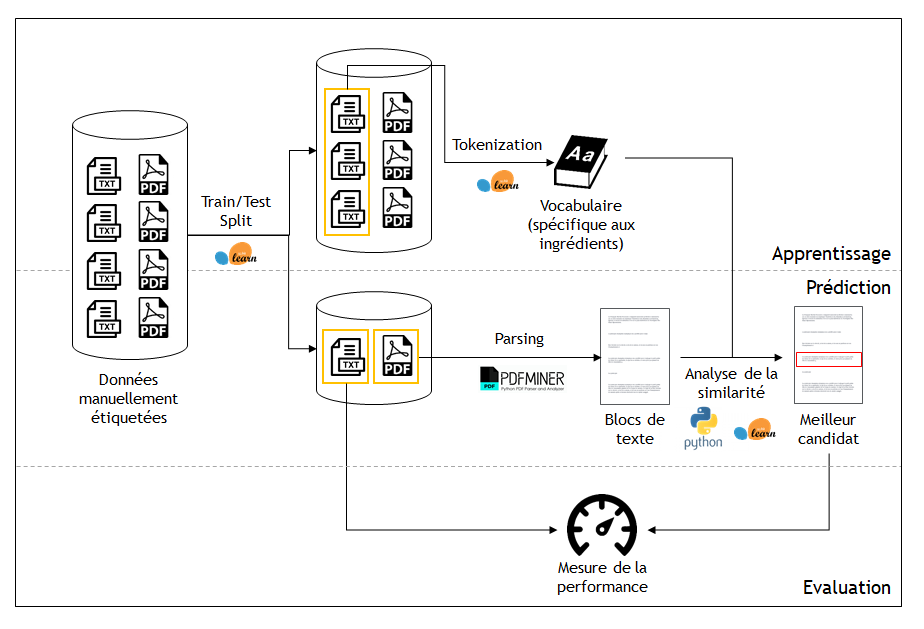
\includegraphics[width=0.9\linewidth]{img/measured_model.png}
        \end{center}
        \caption{Illustration de la méthodologie de mesure de la performance}
        \label{fig:measured_model}
    \end{figure}     

        \section{Accuracy}
        
        La métrique qui tombe le plus sous le sens est l'accuracy (on utilisera le terme anglais pour éviter les confusions avec la notion de \og precision \fg telle qu'elle est utilisée par exemple dans le f1-score).
        On mesure simplement la proportion de prédictions qui sont égales à la ground truth.
        La méthodologie utilisée est détaillée dans le notebook \og Mesure de la performance \fg présenté en annexe \mref{code:performance_measurement}.

            \subsection{Approche naïve}

                \subsubsection{Description de cette approche}

                L'approche \og naïve \fg consiste simplement à mesurer la proportion de textes prédits strictement égaux à la ground truth.
                Or, comme cela a été vu précédemment : 
                \begin{itemize}
                    \item les règles d'étiquetage manuel, détaillées à l'annexe \mref{annotation_rules}, montrent que des transformations sont parfois appliquées au contenu des listes d'ingrédients des pièces jointes avant d'établir la ground truth
                    \item les textes à comparer sont longs (jusqu'à quelques centaines de caractères), cf. \reftable{tbl:GT_prediction_sample}
                    \item la mise en forme, en particulier les retours à la ligne, ne sont pas positionnés aux mêmes endroits. Dans le parsing des documents pdf, lorsque le texte revient à la ligne après avoir atteint le bord de la page, on a un retour à la ligne. Ce comportement n'a pas été reproduit dans l'établissement de la ground truth
                    \item le découpage en blocs de texte, de manière simple, produit des textes qui ne sont pas toujours le reflet du contenu spatialisé de ce document (cf. l'exemple donné à la section \mref{blocks_examples}, et la fiche technique associée en annexe \mref{ex:FT_meltrappeur})
                \end{itemize}
                On s'attend donc à avoir une \og accuracy naïve \fg faible.

                \subsubsection{Les résultats obtenus}

                Comme présenté dans notebook \og Analyse de la performance \fg (cf. annexe \mref{code:performance_measurement}), les résultats obtenus sont conformes à l'attendu : l'accuracy est très faible.
                Elle vaut 1\% (1 échantillon sur 100 produits) lorsqu'on la mesure sur l'échantillon de test après entraînement sur l'échantillon d'entraînement.
                Le seul produit pour lequel la liste d'ingrédients a été correctement identifiée porte les ingrédients suivants.
                \begin{quotation}
                    Sirop de glucose, sucre, eau, stabilisants (E440i, E440ii, E415), acidifiants (E330, E450i), conversateur (E202).
                \end{quotation}
                Si on effectue une cross-validation sur l'ensemble des données étiquetées, en appliquant un découpage en 10 folds, on obtient une accuracy moyenne de $1.80\% \pm 1.89\%$.

                \subsubsection{Nécessité d'améliorer cette métrique}
                On a vu que l'accuracy calculée de manière naïve porte un jugement sévère sur la performance du modèle.
                Par exemple, à la troisième ligne de la \reftable{tbl:GT_prediction_sample}, on voit bien que la liste d'ingrédients prédite est identique à la ground truth, si ce n'est qu les retours à la ligne ne sont pas positionnés exactement au même endroit.
                Comme on souhaite pouvoir ajuster le modèle, il est nécessaire d'avoir une métrique de mesure de la performance qui soit plus précise.

            \subsection{Avec du \og text-postprocessing \fg}
            \label{text_postprocessing}

                \subsubsection{Le principe}
                Afin de pallier ces problèmes de mise en forme de texte, on assouplit un peu les contraintes par rapport à l'égalité stricte.
                En effectuant un traitement de text processing, à la fois sur la ground truth et les résultats du modèle, on va comparer des textes un peu plus \og standardisés \fg.
                Les traitements effectués sont les suivants :
                \begin{itemize}
                    \item On passe le texte en minuscules
                    \item On retire la ponctuation
                    \item On remplace tous les \og whitespaces \fg (retours à la ligne, espaces multiples, tabulations, \dots) par des espaces simples
                    \item On retire les accents
                \end{itemize}
                L'ensemble de ces transformations sont faites en utilisant les fonctionnalités proposées par le CountVectorizer de la bibliothèque scikit-learn (cf. le notebook en annexe \mref{code:performance_measurement} et le module pimest inclus en annexe \mref{code:pimest}).

                \subsubsection{Les résultats}

                Si on évalue cette nouvelle accuracy avec le text processing, sur l'échantillon d'entraînement après entraînement sur l'échantillon d'entraînement, on obtient une accuracy de 14\% (14 listes d'ingrédients correctement prédites sur 100).
                Ces 14 listes d'ingrédients sont présentées à la \reftable{tbl:GT_postprocessed_corrects}.

               {\renewcommand{\arraystretch}{1.5}%
                \begin{table}
                    \begin{spacing}{1.0}
                    \begin{center}
                    {\scriptsize
                    \begin{tabular}{p{7cm}p{7cm}}
\toprule
                                                                                                                                                                                                                                                                                                                                   Liste d'ingrédients cible &                                                                                                                                                                                                                                                                                                                                        Liste d'ingrédients prédite \\ \hline
\midrule
                                                                                                                                                                                                                                                                          Gésier de dinde émincé 50\%, graisse de canard 47\%, sel, arômes naturels de poivre. &                                                                                                                                                                                                                                                                            Gésier de dinde émincé 50\%,  graisse de canard 47\%, sel, arômes naturels de poivre.  \newline   \\ \hline
 Edulcorants sorbitol, isomalt, sirop de maltitol, aspartame, mannitol, sel d'aspartame-acesulfame, acesulfame-k, sucralose; gomme base (contient de la lecithine de SOJA), aromes, epaississant gomme arabique, humectant glycerol, colorant E171, agent d'enrobage cire de carnauba, colorant E163, antioxygene BHA. Contient une source de PHENYLALANINE. &  Edulcorants sorbitol, isomalt, sirop de maltitol, aspartame, mannitol, sel d'aspartame-acesulfame, acesulfame-k, sucralose;  \newline gomme base  (contient de la lecithine de SOJA), aromes, epaississant gomme arabique, humectant glycerol, colorant E171,  \newline agent d'enrobage cire de carnauba, colorant E163, antioxygene BHA. Contient une source de PHENYLALANINE.  \\ \hline
                                                                                                                                                                                                        mini poivrons jaunes, eau, sucre, sel, affermissant chlorure de calcium : E509, acidifiant : acide citrique, vinaigre, antioxydant : vitamine C E330 &                                                                                                                                                                                                          mini poivrons jaunes, eau, sucre, sel, affermissant chlorure de  \newline calcium : E509, acidifiant : acide citrique, vinaigre, antioxydant :  \newline vitamine C E330  \\ \hline
                                                                    Farine de BLE, huile de colza non hydrogénée, OEUFS de poules élevées en plein air (21\%), sucre, stabilisant : glycérol, sirop de glucose-fructose, émulsifiant : mono- et diglycérides d'acides gras, poudres à lever : diphosphates et carbonates de sodium (BLE), fécule, sel, arôme. &                                                                         Farine de BLE, huile de colza non hydrogénée, OEUFS de poules élevées en plein air (21\%), sucre, stabilisant : glycérol, sirop de glucose-fructose, émulsifiant : mono- et diglycérides d'acides gras,  \newline poudres à lever : diphosphates et carbonates de sodium (BLE), fécule, sel, arôme. \\ \hline
                                                                                                                              Pommes de terre 59,5 \% - Céleris 40 \% - Amidon de maïs - Sirop de glucose de maïs - Huile de colza - Emulsifiants : E322, E471 - Stabilisant : E450i - Curcuma - Conservateur : E223 - Antioxydant : E304 - Acidifiant : E330. &                                                                                                                                   Pommes de terre 59,5 \% - Céleris 40 \% - Amidon de maïs - Sirop de glucose de maïs - Huile de colza - Emulsifiants : E322, E471 - Stabilisant : E450i  \newline - Curcuma - Conservateur : E223 - Antioxydant : E304 - Acidifiant : E330. \\ \hline
                                                                                                                                                                                                                                                                                                                                                      <rien> &                                                                                                                                                                                                                                                                                                                                                             <rien> \\ \hline
                                                      Amidon de maïs* - Lait écrémé* - Sel - Fécule de pomme de terre* - Tomate* - Oignon* - Arômes naturels - Poivres* 3 \% (poivre vert*, poivre blanc*, poivre noir*) - Huile de tournesol* - Extrait de levure* - Sucre caramélisé* - Ail* - Maltodextrine de maïs*. \newline * issus de l'agriculture biologique &                                                          Amidon de maïs* - Lait écrémé* - Sel - Fécule de pomme de terre* - Tomate* - Oignon* - Arômes naturels - Poivres* 3 \% (poivre vert*, poivre blanc*,  \newline poivre noir*) - Huile de tournesol* - Extrait de levure* - Sucre caramélisé* - Ail* - Maltodextrine de maïs*.  \newline * issus de l’agriculture biologique \\ \hline
                                                                                                                                                             Farine de FROMENT, poudre de LACTOSERUM, sucre, poudre d'OEUF entier, poudres à lever: (E450, E500), matière grasse LAITIERE, sel. \newline Peut contenir des traces de : soja, fruits à coques, lupin. &                                                                                                                                                                  Farine de FROMENT, poudre de LACTOSERUM, sucre, poudre d'OEUF entier, poudres à lever: (E450,  \newline E500), matière grasse LAITIERE, sel. \newline Peut contenir des traces de : soja, fruits à coques, lupin. \\ \hline
                                                                                                                                                        Eau, maltodextrine, sel, arômes, sucre, arôme naturel de citronnelle, amidon modifié, ail en poudre, épices (combava, curcuma), extraits d'épices (gingembre, poivre), stabilisant (gomme xanthane). &                                                                                                                                                          Eau, maltodextrine, sel, arômes, sucre, arôme naturel de citronnelle, amidon modifié, ail en poudre, épices (combava, curcuma), extraits  \newline d'épices (gingembre, poivre), stabilisant (gomme xanthane).    \\ \hline
                                                                                        OEUFS, farine de BLE, sucre, amidon de BLE, stabilisants: sorbitols- glycérol, cacao maigre en poudre (3,5\%), émulsifiants: E472b - E477, poudres à lever: E450 - E500, sirop de glucose, LAIT écrémé en poudre, sel, conservateur: E202, épaississant: E410, arôme. &                                                                                             OEUFS, farine de BLE, sucre, amidon de BLE, stabilisants: sorbitols- glycérol, cacao maigre en poudre (3,5\%), émulsifiants: E472b - E477, poudres à lever: E450 - E500, sirop de glucose, LAIT  \newline écrémé en poudre, sel, conservateur: E202, épaississant: E410, arôme. \\ \hline
                                                                                                                                                                                                                                           Sirop de glucose, sucre, eau, stabilisants (E440i, E440ii, E415), acidifiants (E330, E450i), conversateur (E202). &                                                                                                                                                                                                                                                  Sirop de glucose, sucre, eau, stabilisants (E440i, E440ii, E415), acidifiants (E330, E450i), conversateur (E202). \\ \hline
                                                                                                                                                                                                                                                                                 Flageolets verts. Jus : eau, sel, affermissant : chlorure de calcium (E509) &                                                                                                                                                                                                                                                                                       Flageolets verts. Jus : eau, sel, affermissant : chlorure de calcium (E509)  \\ \hline
                                                                                                                                                                                                                                                      Carottes, eau, sucre, sel, vinaigre d'alcool, acidifiant : acide lactique. Présence fortuite de CELERI &                                                                                                                                                                                                                                                             Carottes, eau, sucre, sel, vinaigre d’alcool, acidifiant : acide lactique. Présence fortuite de CELERI \\ \hline
                                                                                                                                               Légumes 43,2 \% (pomme de terre, oignon, carotte, tomate, poireau) - Amidon modifié de pomme de terre - Extrait de levure - Sirop de glucose de maïs - Huile de colza - Sucre - Arôme naturel - Ail - Curcuma. &                                                                                                                                                    Légumes 43,2 \% (pomme de terre, oignon, carotte, tomate, poireau) - Amidon modifié de pomme de terre - Extrait de levure - Sirop de glucose de maïs -  \newline Huile de colza - Sucre - Arôme naturel - Ail - Curcuma. \\ \hline
\bottomrule
\end{tabular}

                    }
                    \caption{Prédictions identifiées comme correctes après postprocessing}
                    \label{tbl:GT_postprocessed_corrects}
                    \end{center}
                    \end{spacing}
                \end{table}
                }

                De la même manière que précédemment, si on fait une cross-validation sur l'ensemble des données manuellement étiquetées, on obtient une accuracy de $16.60\% \pm 3.35\%$.

                \subsubsection{Les limites de cette métrique}

                Cette métrique est déjà plus intéressante que l'approche naïve, mais elle a quand même un défaut majeur : elle a une vision encore trop binaire des résultats.
                En effet, que le texte soit identique à un préfixe près (cf. la quatrième ligne de la \reftable{tbl:GT_prediction_sample}), ou qu'il n'ait rien à voir (d'autres exemples sont présents dans cette même table), elle considèrera la prédiction comme erronée.
                Or, il est important d'identifier les cas où le modèle s'est complètement trompé par rapport à ceux où il a quand même identifié le bon bloc contenant les ingrédients.

        \section{Fonctions de \og similarité \fg spécifiques}

        On peut définir des fonctions de similarité, qui permettent d'être plus fin qu'une simple évaluation binaire du résultat du modèle.
        Cela permet de prendre plus finement en compte les cas où le modèle a identifié un bloc très similaire à la ground truth.
        On va pour cela s'appuyer sur diverses métriques permettant de mesurer l'écart entre des chaînes de caractères.
        \`{A} chaque fois, on définira une fonction de scoring qui sera une similarité : \og higher is better \fg.
        De plus, elles seront normées pour prendre leurs valeurs entre 0 (chaînes de caractères totalement différentes) et 1 (chaînes identiques), ce qui permettra d'exprimer ces métriques en pourcentage.
        Ces similarités seront calculées après application du text-postprocessing, comme décrit à la section \mref{text_postprocessing}.
        L'ensemble de ces similarités seront calculées sur les caractères (on pourrait envisager de les calculer sur les mots).

            \subsection{Similarité basée sur la distance de Levenshtein}

            La distance de Levenshtein~\cite{levenshtein_wiki}  entre deux chaînes de caractères est la distance d'édition pour passer de l'une à l'autre en prenant en compte les transformations suivantes :
            \begin{itemize}
                \item insertion d'un caractère 
                \item suppression d'un caractère
                \item substitution d'un caractère par un autre
            \end{itemize}
            Cette distance possède les caractéristiques suivantes : 
            \begin{itemize}
                \item elle peut se calculer entre deux chaînes de longueur différentees
                \item elle a pour minimum 0 (si et seulement si les deux chaines sont identiques)
                \item a pour majorant la longueur de la plus longue des deux châines
            \end{itemize}
            Pour construire une fonction de similarité telle que présentée en introduction de cette section, on appliquera la transformation suivante : 
            \[sim_{lev}(s_{1}, s_{2}) = 1 - \frac{dist_{lev}(s_{1}, s_{2})}{max(len(s_{1}), len(s_{2}))}\]
            en notant $dist_{lev}$ la distance de Levenshtein, $len(s)$ la longueur de la chaîne $s$, et $s_{1}$ et $s_{2}$ les chaînes de caractères à comparer.
            Par exemple, la distance entre les chaînes \og rateaux \fg et \og chameau \fg vaut 4 :
            \begin{itemize}
                \item substitution du \og r \fg par un \og c \fg
                \item insertion du \og h \fg
                \item substitution du \og t \fg par un \og m \fg
                \item suppression du \og x \fg
            \end{itemize}

            \subsection{Similarité basée sur la distance de Damerau-Levenshtein}

            La distance de Damerau-Levenshtein~\cite{damerau_levenshtein_wiki} est une variante de la distance de Levenshtein.
            Elle calcule également une distance d'édition, mais en ajoutant une transformation possible : l'interversion de deux caractères successifs.
            Les transformations possibles pour cette transformation sont :
            \begin{itemize}
                \item insertion d'un caractère 
                \item suppression d'un caractère
                \item substitution d'un caractère par un autre
                \item interversion de deux caractères successifs
            \end{itemize}
            Ses caractéristiqes sont les mêmes que la distance de Levenshtein (minimum, maximum) ; et elle est toujours inférieure ou égale à la distance de Levenshtein.
            On convertit cette distance en similarité de la même manière que la distance de Levenshtein.

            \subsection{Similarité de Jaro}
            
            La similarité de Jaro~\cite{jaro_wiki} est une fonction permettant de mesurer une similarité entre 0 (chaînes complètement différentes) et 1 (chaînes parfaitement identiques).
            L'heuristique derrière cette similarité est de considérer qu'entre deux chaînes, un caractère est \og correspondant \fg (\og matching \fg) s'il est déplacé d'au moins de la moitié de la longueur de la plus longue des deux chaînes.
            On compte         
            Sur des chaînes longues de quelques dizaines de caractères, la quasi-totalité des caractères seront \og correspondants \fg.
            Elle est en général plutôt adaptée à des comparaison de chaînes courtes telles que des noms propres ou des mots de passe.

            \subsection{Similarité de Jaro-Wrinkler}
            
            La similarité de Jaro-Winkler~\cite{jaro_winkler_wiki} est une variante de la similarité de Jaro.
            Elle possède la même heuristique que la distance de Jaro, avec en plus comme caractéristique de donner un poids plus important aux 4 caractères qui font le début de la chaîne de caractères.
            Cette métrique est encore moins adaptée au cas d'usage que la précédente.

            \subsection{\'{E}valuation de ces similarités sur la ground truth}

            Les résultats de l'évaluation de chacune de ces similarités sont présentés à la \reftable{tbl:similarities_result}.
            \begin{table}[htbp]
                \begin{center}
                \begin{tabular}{lcc}
\toprule
{} & train/test set & cross validation \\
\midrule
\textbf{Levenshtein        } &         48.86\% &  49.79\% +/-3.73\% \\
\textbf{Damerau-Levenshtein} &         48.86\% &  49.80\% +/-3.72\% \\
\textbf{Jaro               } &         63.56\% &  62.78\% +/-3.28\% \\
\textbf{Jaro-Winkler       } &         65.67\% &  64.40\% +/-3.50\% \\
\bottomrule
\end{tabular}

                \caption{\'{E}valuation du modèle en utilisant les métriques de similarité}
                \label{tbl:similarities_result}
                \end{center}
            \end{table}
            On constate que :
            \begin{itemize}
                \item les similarités de Levenshtein et Damerau-Levenshtein donnent des résultats identiques
                \item les similarités de Jaro et de Jaro-Winkler donnent des évaluations très généreuses de la performance du modèle, comme on pouvait s'y attendre sur la base de textes longs
            \end{itemize}

            \subsection{Décision sur la métrique à utiliser et illustration}
            
            Les similarités de Jaro et Jaro-Winkler sont abandonnées car non pertinentes pour notre cas d'usage, qui se base sur des textes de plusieurs dizaines de caractères.
            Les similarités de Levenshtein et Damerau-Levenshtein donnant des résultats identiques, on choisira plutôt la distance de Levenshtein car son implémentation en C (bibliothèque python-Levenshtein) semble plus performante que celle en C++ de la bibliothèque Jellyfish.

            Des exemples du début, du milieu et du bas du classement en termes de similarité de Levenshtein sur le jeu de test, après entraînement sur le jeu d'entraînement, sont présentés à la \reftable{tbl:similarity_illustration}.
            \begin{table}[htbp]
                \begin{center}
                {\tiny
                \begin{tabular}{p{5cm}p{5cm}cccc}
\toprule
                                                                                                                                                                                                                                                              Listes d'ingrédients cibles &                                                                                                                                                                                                                                                                                             Listes d'ingrédients prédites &     Lev & Dam-Lev &    Jaro & Jaro-Win \\ \hline
\midrule
                                                                                                                                                                                                       Gésier de dinde émincé 50\%, graisse de canard 47\%, sel, arômes naturels de poivre. &                                                                                                                                                                                                                                   Gésier de dinde émincé 50\%,  graisse de canard 47\%, sel, arômes naturels de poivre.  \newline   & 100.00\% & 100.00\% & 100.00\% &  100.00\% \\ \hline
                                                                                                                                     mini poivrons jaunes, eau, sucre, sel, affermissant chlorure de calcium : E509, acidifiant : acide citrique, vinaigre, antioxydant : vitamine C E330 &                                                                                                                                                                 mini poivrons jaunes, eau, sucre, sel, affermissant chlorure de  \newline calcium : E509, acidifiant : acide citrique, vinaigre, antioxydant :  \newline vitamine C E330  & 100.00\% & 100.00\% & 100.00\% &  100.00\% \\ \hline
 Farine de BLE, huile de colza non hydrogénée, OEUFS de poules élevées en plein air (21\%), sucre, stabilisant : glycérol, sirop de glucose-fructose, émulsifiant : mono- et diglycérides d'acides gras, poudres à lever : diphosphates et carbonates de sodium (BLE), fécule, sel, arôme. &                                Farine de BLE, huile de colza non hydrogénée, OEUFS de poules élevées en plein air (21\%), sucre, stabilisant : glycérol, sirop de glucose-fructose, émulsifiant : mono- et diglycérides d'acides gras,  \newline poudres à lever : diphosphates et carbonates de sodium (BLE), fécule, sel, arôme. & 100.00\% & 100.00\% & 100.00\% &  100.00\% \\ \hline
                                                                                                                                                                                                                                                               Pommes de terre, eau, sel. &                                                                                                                                                                                                                                  Anhydride sulfureux et sulfites en  \newline concentrations de plus de 10 mg/kg  \newline exprimé en SO2 &  15.48\% &  15.48\% &  48.29\% &   48.29\% \\ \hline
%                                                                                                                                                                                                                                           Débris de truffes d'hiver, jus de truffes, sel &                                               \newline Origine Truffes et Sel          :           France et/ou Espagne  \newline   \newline Traçabilité                            :          Chaque lot est enregistré et identifié.  \newline   \newline Caractéristiques organoleptiques : Débris de couleur hétérogène (marron à noir)  sans colorant, dans  &  14.97\% &  14.97\% &  47.87\% &   47.87\% \\ \hline
                                                                                                                                                                                                                                                                     AMANDES décortiquées &                                                                                                       Valeur énergétique :  \newline      Matières grasses :   \newline           dont ac gras saturés :  \newline      Glucides :  \newline           dont sucres :   \newline      Fibres alimentaires :        Dietary fibre  \newline      Protéines :  \newline      Sel :   &  12.80\% &  12.80\% &  46.93\% &   46.93\% \\ \hline
                                                                                                                                                                                                                                              Poire 99,9\%, antioxydant: acide ascorbique. &  Ce produit est une purée de fruits obtenue à partir des parties comestibles des fruits (après broyage et sans  \newline concentration notable). \newline Ce produit est sans sucres ajoutés: il contient uniquement les sucres naturellement présents dans les fruits. \newline La purée présente une texture homogène et légèrement granuleuse. &   9.67\% &   9.67\% &  43.73\% &   43.73\% \\ \hline
                                                                                                                                                                                                                                                                 100\% haricots blancs bio &                              Les légumes secs sont mis en avant par tous les nutritionnistes pour leurs apports en protéines et fibres. Ils s’inscrivent parfaitement  \newline dans le PNNS.  \newline Les légumes secs bio bénéficient également d’une agriculture résonnée et donne des garanties en termes de développement durable.  &   6.62\% &   6.62\% &  35.47\% &   35.47\% \\ \hline
                                                                                                                                                                                                                                                                                   Persil &                                                                                                                                                                         Céréales contenant du gluten (à savoir blé, seigle, orge, avoine, épeautre, Kamut ou leurs souches hybrides) \newline et Produits à base de ces Céréales. &   4.55\% &   4.55\% &  50.76\% &   50.76\% \\ \hline
\bottomrule
\end{tabular}

                }
                \caption{Illustration de l'évaluation du modèle à l'aide des métriques de similarité}
                \label{tbl:similarity_illustration}
                \end{center}
            \end{table}

    \chapter{Transfer learning}
        
        \section{Principe du pré-entraînement}
        
        Expliquer qu'il s'agit d'une approche hybride des 2 modèles précédents
        On effectue une entraînement à la fois sur une partie des listes d'ingrédients du PIM, et sur une partie des données étiquetées.
        On vérifie ensuite, uniquement sur 

        \section{Illustration de l'impact sur la performance}

        Ici, on montre l'impact sur la performance, du fait d'intégrer des listes d'ingrédients.
        On met en abscisse le nombre de listes d'ingrédients qu'on ajoute, et en ordonnée la performance du modèle (avec barre d'erreurs, via cross validation).
        On regarde si l'effet est positif : cela montrera s'il est intéressant d'avoir plus de données.
        On regarde si on observe une saturation : cela montrera si on a déjà suffisamment de données sous formes de listes d'ingrédients dans le PIM, ou bien si ce serait intéressant d'en acquérir plus.

    \chapter{Hyperparameter tuning}
            
    On peut, dans l'optique d'améliorer la performance du modèle, ajuster certains paramètres et d'évaluer l'impact via une grid search.
    On fera tourner sur le modèle avec transfer learning.

        \section{Les paramètres ajustables}

            \subsection{La prise en compte des \og n-grams \fg dans la tokeinzation}

            On peut utiliser les n-grams lors de la tokenisation.

            \subsection{L'application de \og n-grams \fg de blocs}

            Voir si dans la recherche du meilleur candidat, on s'autorise la constitution de \og n-grams \fg de blocs.

            \subsection{L'utilisation d'expressions régulières dans le split des blocs}

            Voir si certaines expressions régulières pour splitter les blocs procurent de meilleurs résultats.

            \subsection{Applications d'autres fonctions de similarité}

            Voir l'impact d'utiliser d'autres manières de calculer la similarité.

            1 - autre chose que la similarité cosinus (fonction du nombre de mots du bloc et de la proportion de mots issus du vocabulaire des ingrédients)

            2 - en appliquant du TF et du TF-IDF

        \section{Application d'une grid search}

        Illustrer ici les résultats d'une grid search ou d'une random search si trop gourmand.